\documentclass[parskip=half*,fontsize=12pt,abstract]{scrartcl}
\usepackage{scrhack}
\usepackage{geometry}
\geometry{a4paper, top=2cm, left=2.5cm, right=3cm, bottom=2cm,footskip=1cm}
\usepackage{setspace}

\usepackage[utf8]{inputenc}
\usepackage[T1]{fontenc}
\usepackage{lmodern}
\usepackage[ngerman]{babel}
\usepackage[ngerman=ngerman-x-latest]{hyphsubst}
\usepackage{amsmath}
\usepackage[autostyle=true, german=quotes]{csquotes}
\PassOptionsToPackage{hyphens}{url}
\usepackage[pdfpagelabels]{hyperref}
\usepackage[nottoc,notlot,notlof]{tocbibind}
%\usepackage[htt]{hyphenat} 

\usepackage{graphicx}
\usepackage{pdfpages}
\usepackage{tikz}
\usepackage{todonotes}
\usepackage{mdframed}
\usepackage{changepage}
\usepackage{listings} %Für Code
\usepackage[german,onelanguage,boxed]{algorithm2e}%Für Pseudocode
\usepackage{enumitem}
\usepackage{mdwlist}
\usepackage{tcolorbox}
\usepackage{tabularx}
\usepackage{longtable}

\newcolumntype{L}[1]{>{\raggedright\arraybackslash}p{#1}} % linksbündig mit Breitenangabe
\newcolumntype{C}[1]{>{\centering\arraybackslash}p{#1}} % zentriert mit Breitenangabe
\newcolumntype{R}[1]{>{\raggedleft\arraybackslash}p{#1}} % rechtsbündig mit Breitenangabe

\newenvironment{heft}[1]{\begin{mdframed}\textbf{Hefteintrag: #1}\newline}{\end{mdframed}}
\newenvironment{tafel}[1]{\begin{mdframed}\textbf{Tafelanschrieb: #1}\newline}{\end{mdframed}}
\newenvironment{pseudocode}{\begin{algorithm}[H]
\SetKwFor{ForEach}{Wiederhole für alle}{}{Ende}
}{
\end{algorithm}}

\newcommand{\syso}[1]{\texttt{#1}}
\newcommand{\zitat}[1]{\enquote{\textit{#1}}}

\definecolor{light-gray}{gray}{0.95}
\newcommand{\class}[1]{\colorbox{light-gray}{\texttt{#1}}}

\begin{document}
\onehalfspacing
\pagestyle{empty}
\begin{titlepage}
{\centering
Ludwig-Maximilians-Universität München\\
Fakultät für Mathematik, Informatik und Statistik\\
Department Institut für Informatik
\vspace{1.5cm}

{\huge\bfseries	Entwicklung eines neuartigen Tower Defense Spieles}
\Large
\vspace{1.5cm}

vorgelegt von: Benjamin Knorr \\
MatrikelNr: 10967090\\[1cm]
\textbf{Ausarbeitung\\
 Praktisches Programmieren}\\[1cm]
Betreuende Dozentin: \\
Paola Maneggia

\vfill
}
Schopenhauerstraße 66, 80807 München \\
Knorr.Benjamin@campus.lmu.de\\
München, den \today
\end{titlepage}

\tableofcontents 
\newpage
\pagestyle{plain}

\section{Projektidee} % (fold)
\label{sec:projektidee}



\subsection{Bisherige Tower Defense Spiele}

Das Tower Defense Genre..... Das Grundkonzept ist dabei immer, dass der Spieler mehrere Wellen an KI-Gegnern, sogenannte \enquote{Creeps}, auf einer Karte davon abhalten muss, bestimmte Ziele zu erreichen. Dazu kann er Türme platzieren, die die Creeps töten. In den meisten Fällen handelt es sich um eher kleinere Spiele, wie Browser-, Flash- oder Mobile Games und auch die ersten bekannteren TD Spiele sind als Custom Maps im Warcraft oder StarCraft MapEditor entstanden und haben daher kein großes Entwicklerteam im Hintergrund. Der Umfang war damit für das eigene Projekt gut abschätzbar und der vorgesehenen Bearbeitungszeit angemessen. Vereinzelt wurde das Spielprinzip aber auch in größeren Produktionen, wie \todo{\dots}, aufgegriffen, was die Erweiterbarkeit des Ansatzes zeigt. Es existieren bereits einige Spielvariationen, über die im Folgenden exemplarisch ein Überblick gegeben werden soll.

\paragraph{Klassisches Spiel}
In der häufigsten (da einfachsten) Spielimplementierung bewegen sich die Creeps auf einem vordefinierten Pfad und die Türme werden entlang des Pfades frei oder auf bestimmten Knotenpunkten positioniert.Typischer Weise gibt es unterschiedliche Türme und verschiedene Creep-Arten. Zum Teil haben diese auch Spezialfähigkeiten, wie fliegende Creeps (folgen also nicht dem Pfad, sondern bewegen sich auf direkter Linie zum Ziel) bzw. Türme, die besonders gut gegen Bodeneinheiten oder gegen fliegende Einheiten sind. Häufig werden die Creeps auch in ihrer Geschwindigkeit variiert und es existieren Türme, die Creeps verlangsamen sowie Creeps die dagegen immun sind.  Diese Spiele rücken besonders das taktisch geschickte Kombinieren der verschiedenen Türme und das Aufrüsten an entscheidenden Knotenpunkten in den Fokus des Spielerlebnisses.

\missingfigure{Screenshot of normal Game}

\paragraph{Mazing Tower Defense}
Eine weitere Variante sind die \enquote{Mazing Tower Defense Spiele}, in denen die Creeps sich nicht auf einem vordefinierten Pfad bewegen, sondern der Spieler mit den Türmen eine Labyrinth artige Struktur baut, durch die die Creeps dann durchlaufen. Das erste Spiel dieser Art und daher prototypisch ist \enquote{Desktop Tower Defense} aus dem Jahr 2007 von Paul Preece, das bereits in den ersten zwei Monaten 15 Millionen Mal gespielt wurde und inzwischen durch eine Erneuerung als Facebook Anwendung noch populärer geworden. Das Spielprinzip erweitert das normale Spiel um eine strategische Planung der Kreaturenführung durch das Labyrinth um die Türme möglichst effektiv aufrüsten zu können. Die Spielelemente sind dabei weiterhin die klassischen Kreaturenarten und Turmvarianten.

\missingfigure{Screenshot of Desktop Tower Defense}

\paragraph{Andere Varianten} Es existieren noch viele weitere Varianten wie das sehr erfolgreiche Plants vs Zombies, bei dem die Creeps (=Zombies) die Türme angreifen und keine Wegfindung implementiert ist, das aber eine sehr große Vielfalt an verschiedenen Gegnern und Strategien einbringt, oder auch Multiplayer Spiele. Diese waren jedoch keine Inspirationsquelle für das eigene Projekt und werden daher nicht genauer betrachtet.

\subsection{Neuer Ansatz im eigenen Projekt}

Mazing Tower Defense erweiterte das klassische Spiel um die Herausforderung ein möglichst effektives Labyrinth zu bauen. Dabei ist jedoch die Wegsuche der Creeps optimal, wodurch zwar Labyrinthe aber keine Irrgärten entstehen. Denn Verzweigungen und Sackgassen nehmen nur unnötigen Platz weg und die Creeps werden nie in diese Bereiche hineinlaufen. Die Spielidee für dieses Projekt ist, dass die Anlage eines komplizierten Irrgartens dem Spieler einen Vorteil für das Spiel bringen soll. Um dies zu ermöglichen wurde die Prämisse aus dem Spiel genommen, dass die Kreaturen einen allwissenden Überblick über das Labyrinth haben. Stattdessen sollten sie das Labyrinth erkunden müssen. Diese Variation hatte viele Designentscheidungen zur Folge, die im Folgenden kurz vorgestellt werden.

\missingfigure{Vergleich Labyrinth in Tower Defense vs. Irrgarten}

\paragraph{State der Kreaturen} In den bisherigen Spielvarianten benötigten die Kreaturen keine eigene Repräsentation der Welt. Dagegen müssen die Creeps sich nun individuell auf Grundlage ihres bisherigen Wissens über die Welt bewegen. Ein wichtiges Spielelement ist daher die Klasse \lstinline{VisitedMap}, mit der jede Kreatur in einem zweidimensionalen Enum-Array dieses Wissen speichert. Andererseits sollen die Kreaturen auch über eine gewisse Intelligenz verfügen und nicht alle in die selbe Sackgasse laufen. Das gelingt durch simulierte Besprechungen zwischen den Kreaturen Die Karten müssen also effizient synchronisierbar sein. \todo{Link auf später}

\paragraph{Wegfindung} Die effiziente Wegfindung ist ebenfalls schwieriger: Während bei normalen TD Spielen gar keine Berechnung notwendig ist und bei Mazing TD ein A*-Algorithmus effizient den kürzesten Weg von allen Kartenpunkten zum Ziel berechnen kann, muss der Algorithmus hier noch weiter abgewandelt werden, da die Creeps nicht nur ein Ziel haben. Es muss daher für jeden Creep ein eigenes Ziel ausgewählt werden, was zum Beispiel durch wiederholte Nearest-Neighbor-Suche umgesetzt werden kann.

\paragraph{Variationsmöglichkeiten} Dadurch, dass die Kreaturen ihre eigene Wegfindung haben und Absprachen treffen, ergeben sich neue Möglichkeiten der Variation der Creeps. Beispielsweise wurden Figuren implementiert, die sich nur zufällig bewegen, andere versuchen jedes Feld der Welt zu besuchen. Weitere Möglichkeiten wären Kreaturen, die tatsächlich sehen können und damit z.B. größere Flächen direkt durchqueren, oder Kreaturen die andere dirigieren. Auch neue Turmarten, die auf diese Wegfindung Einfluss haben, sind möglich. Als Beispiel wurde dafür ein Amnesie-Turm programmiert, der die Wegsuche der abgeschossenen Creeps eine gewisse Zeit lang zu zufällig ändert.

\paragraph{Labyrinthänderungen} Die für das Genre typischen Echtzeit-Änderungen des Labyrinths sind in der Variante schwieriger an Kreaturen zu kommunizieren. Da die Creeps den Zustand ihrer erkundeten Welt speichern, sind Änderungen in bereits erkundeten Bereichen problematisch. Es gibt mehrere Möglichkeiten damit umzugehen, die in der Entwicklung abgewogen und mit User-Testings betrachtet wurden:
\begin{itemize}
	\item Kreaturen erhalten kein Update über die Welt. Bei dieser Lösung musste ein Verhalten implementiert werden, falls Creeps denken es gäbe keinen Ausweg. Typischer weise greifen eingesperrte Figuren die Türme an oder rennen darüber, was in der eigenen Variante so implementiert wurde. Das User Feedback zeigte, dass das Verhalten der Creeps insb. wegen der Kommunikation nicht nachvollziehbar ist.
	\item Kreaturen erhalten ein Update, falls sie den Bereich bereits erkundet hatten. Dies führte in User-Testings zu Strategien gegen das Spielprinzip, bei denen zwei Türme auf verschieden Seiten der Karte immer abwechselnd neu gebaut und später wieder abgerissen wurden, sodass die Kreaturen immer von einem Ende zum anderen laufen mussten.
	\item Türme können gar nicht abgerissen werden, oder nur wenn kein lebender Creep diesen erkundet hat. Dies schränkt die Möglichkeiten der Spieler zwar ein, ist aber besser verständlich und bleibt dem Spielprinzip treu.
\end{itemize}

% section projektidee (end)
\section{Entwicklungsprozess} % (fold)
\label{sec:entwicklungsprozess}

Bei dem Entwicklungsprozess wurde auf mehrere professionelle Elemente besonderen Wert gelegt. Diese sollen im Folgenden kurz erläutert werden.
\subsection{Werkzeuge} % (fold)
\label{sub:werkzeuge}
\paragraph{Versionsverwaltung} % (fold)
\label{par:versionsverwaltung}
Eine der grundlegendsten Dinge bei der Softwareentwicklung ist ein Versionskontrollsystem. In diesem Projekt wurde dafür \emph{Git} verwendet und in einem Repository auf Github (\url{https://github.com/Knorrke/MazeRunner}) veröffentlicht. Dies ermöglichte zum einen unkompliziert das Arbeiten auf mehreren Geräten. Zum anderen konnte durch das Erstellen neuer Branches seperat an Features entwickelt werden, ohne die Hauptversion während dem Entwicklungsprozess zu verändern. Über Pull Requests wurden die Features dann in den Hauptzweig gemerget.
% paragraph versionsverwaltung (end)

\paragraph{Dependency Managagement} % (fold)
\label{par:dependency_managagement}
Um nicht jedes Mal das Rad neu zu erfinden, ist es oft sinnvoll existierende Bibliotheken zu verwenden. Damit das Projekt leicht auf anderen PCs eingerichtet werden kann, sollte das Einbinden von solchen Abhängigkeiten durch ein Verwaltungssystem geschehen. Dafür wurde \emph{Maven} verwendet, das ebenfalls eine Buildautomatisierung ermöglichte.
% paragraph dependency_managagement (end)

\paragraph{Continuous Integration} % (fold)
\label{par:continuous_integration}
Mit einem Continuous Integration Service (in diesem Fall \emph{Travis CI}) konnte sichergestellt werden, dass die Tests nicht nur auf dem eigenen Gerät funktionieren, sowie dass Pull Requests vollständig funktionsfähig sind bevor sie in den Hauptzweig eingebunden werden. Des Weiteren ließ sich dadurch das Testcoverage Tool \emph{JaCoCo} integrieren (Genaueres siehe \ref{sub:testgetriebene_entwicklung}).
% paragraph continuous_integration (end)
% subsection werkzeuge (end)

\subsection{Testgetriebene Entwicklung} % (fold)
\label{sub:testgetriebene_entwicklung}

Für die Gewährleistung der Funktionalität und Absicherung für Änderungen sind Unit-Tests enorm hilfreich. Sie verkürzen die Zeit zur Fehlersuche, da Fehler direkt mit einem Knopfdruck angezeigt werden können. Außerdem geben sie dem Entwickler Sicherheit bei größeren Strukturänderungen, dass das System danach noch die Anforderungen erfüllt. Das Projekt wurde komplett testgetrieben entwickelt. Diese Methode beschreibt das Vorgehen, vor der Implementierung bereits den Test zu schreiben, also zu definieren wie der Code sich verhalten soll. Anschließend wird dieser Test so einfach wie möglich erfüllt. Dadurch wird sichergestellt, dass nur Code geschrieben wird, der auch wirklich notwendig ist. In einer dritten Phase, dem Refactoring, wird der Code anschließend nochmal bzgl Code-Qualität überarbeitet. Dabei hilft der bereits definierte Test zu überprüfen, ob die Funktionalität nach dem Refactoring immer noch gegeben ist. 

Ein Testcoverage Tool ermöglicht anschließend zu überprüfen, ob auch alle Teile des Codes durch Tests abgedeckt sind. In diesem Projekt liegt die Testabdeckung zur Zeit der Abgabe bei 98\%. Die restlichen 2\% betreffen überwiegend das Loggen von evtl. auftretenden \class{IOExceptions}, die nicht extra für Tests erzeugt wurden.

Um die Tests eines Codeteiles besser von dem Verhalten des restlichen Codes trennen zu können, wurde zudem das Mocking Framework \emph{Mockito} verwendet. Das ermöglicht es, für Klassen und Interfaces eine Art Attrappe zu erzeugen, für die dann konfiguriert werden kann, wie er auf bestimmte Methodenaufrufe mit den korrekten Argumenten reagiert. Zum Einen kann dadurch der zu testende Code besser isoliert werden, weil keine Abhängigkeiten zu anderen Klassen existieren. Es kann aber auch überprüft werden, ob die Aufrufe richtig stattgefunden haben, ob also die Interaktion mit dem Mock-Objekt so ablief, wie erwartet. Dadurch lässt sich auch die Integration in den restlichen Softwareaufbau gut testen.
\missingfigure{Beispielcode von Mockito}
% subsection testgetriebene_entwicklung (end)


\subsection{JavaFX} % (fold)
\label{sub:javafx}
Für die Umsetzung der Benutzeroberfläche wurde JavaFX verwendet, das durch die Abwandlung des Observer-Patterns auch viel Einfluss auf den Softwareentwurf hatte (siehe Kapitel \ref{sub:observer}). Das Framework ermöglichte eine modern wirkende Oberfläche durch viele vorgefertigte Komponenten und zahlreiche verfügbare Erweiterungen, wie z. B. ein Popup-Menü. Dabei wird die Komplexität von Swing für ansprechende Layouts deutlich reduziert und das meiste geschieht für den Programmierer unsichtbar im Hintergrund. Zudem existiert für JavaFX Anwendungen das Projekt \emph{javafxports}, das ermöglicht den gesamten Code ohne große Anpassungen direkt in Mobile Apps zu packen.

Für die testgetriebene Entwicklung ist die View-Programmierung eine Herausforderung. Hierfür konnte jedoch mit \emph{TestFX} (\url{https://github.com/TestFX/TestFX}) ein gutes Framework verwendet werden, das eine schnelle und anschauliche Implementierung von Unit-Tests für JavaFX ermöglicht. Dadurch konnte auch die korrekte Reaktion auf (erwartete) Userinteraktionen überprüft werden.
\missingfigure{Beispielcode von TestFX}
% subsection javafx (end)
% section entwicklungsprozess (end)
\section{Softwaredesign} % (fold)
\label{sec:softwaredesign}

Um den Code leicht erweitern zu können und Fehlern vorzubeugen, ist es wichtig, den Aufbau der Software gut zu strukturieren. Dabei gibt es einige typische Probleme, für die bereits etablierte Lösungen existieren. Diese Design Pattern helfen nicht nur dabei, den Code wartbar zu halten, sondern helfen auch in der Kommunikation mit anderen Entwicklern bei strukturellen Problemen. In diesem Kapitel soll ein Highlevel-Überblick über die Softwarestruktur und verwendete Design Muster gegeben werden.

\subsection{Model View Controller} % (fold)
\label{sub:model_view_controller}
Eines der wohl am weitesten verbreitete Entwurfsmuster ist das Model View Controller Pattern, das auch in dieser Arbeit umgesetzt wurde. Es trennt die verschiedenen Aufgaben einer Software in drei Bereiche auf: Daten und Spiellogik bilden das Modell, das in sich funktioniert und nach außen Schnittstellen bietet, die dann interne Spielprozesse auslösen. Getrennt davon ist die View, deren Aufgabe einzig darin besteht, die Daten aus dem Modell (evtl. gefiltert) dem Spieler anzuzeigen. Diese View ist mit JavaFX geschrieben, wobei die Trennung vom restlichen Code teilweise durch die Verwendung von \emph{FXML} besonders deutlich wird. Die View muss dabei Änderungen aus dem Modell mitbekommen und daraufhin entsprechend anzeigen. Die View stellt zudem Schnittstellen zur Verfügung, um auf bestimmte Useraktivitäten zu reagieren. Diese Schnittstellen verwendet der Controller. Er setzt also Listener auf Komponenten der View für verschiedene User Interaktionen wie Mausklicks, Hovering oder Tastatureingaben. Die Listener sind größtenteils als anonyme Klassen implementiert und rufen bei einer Aktion die entsprechenden Schnittstellen des Modells auf.  
% subsection model_view_controller (end)

\subsection{Observer Pattern} % (fold)
\label{sub:observer}
Im Zusammenspiel mit MVC ist das Observer Pattern eines der wichtigsten. Es ermöglicht eine lose Kopplung zwischen View und Modell, indem sich die View beim Modell als Observer registriert und das Modell bei Änderungen alle Observer benachrichtigt. Dadurch ist gewährleistet, dass das Modell nicht explizit die View kennen muss und so kann die View leichter ausgetauscht werden oder weitere Views (z.B. auch Sounds) angebunden werden, ohne in das Modell einzugreifen. In JavaFX funktioniert die Umsetzung ein wenig anders, nämlich mittels \enquote{Bindings}: Das Modell bietet Properties an, auf denen Listener registriert werden können, die aber auch direkt an Viewausgaben gebunden werden können. Beispielsweise stellt die Geldanzeige im Spiel einen formatierten String der \class{IntegerProperty money} des \class{PlayerModel} dar. Da immer das aktuelle Geld angezeigt werden soll, kann hierfür ein Binding verwendet werden, statt den Umweg über einen Listener zu nehmen.
% subsection observer (end)

\subsection{Game Loop} % (fold)
\label{sub:gameloop}
Eine Game Loop löst das Problem, die Spielzeit mit der Realzeit zu synchronisieren, statt ihren Ablauf von User-Interaktionen (wie bei klassischen EVA), abhängig zu machen oder von der Prozessorgeschwindigkeit abhängig zu sein \cite{gameloopPattern}. Die Implementierung richtet sich nach \cite{gameloopImpl, gameloopImplFX} und verwendet drei Elemente:
\begin{itemize}
	\item \textbf{Synchronisation mit der Realzeit}: Messe wie viel Realzeit seit der letzten Spielzeit Simulation vergangen ist und simuliere ungefähr diese Zeitspanne (Einschränkungen siehe die nächsten zwei Punkte).

	\item \textbf{Feste Zeitschritte}: Eine Frame Rate über 60 Bilder pro Sekunde ist nicht notwendig, daher wird versucht diese Zielrate ungefähr zu erreichen. Kürzere Zeitschritte werden also zusammengefasst, bis \(1/60\) Sekunde zusammenkommen, größere Zeitschritte werden in mehrere 1/60 Sekunden Schritte zerteilt und einzeln simuliert. Dadurch bleibt das Spiel deterministisch -- im Gegensatz zur Verwendung von variablen Zeitschritten.

	\item \textbf{Begrenzte Zeitschritte}: Ist der Prozessor zu langsam, um eine Iteration in \(1/60\,s\) auszuführen, ist bei der nächsten Iteration mehr Zeit vergangen, wodurch er mehr Zeitschritte machen muss, die wieder länger dauern, etc. Um diese Spirale zu verhindern, wird die vergangene Zeit auf eine bestimmte Länge beschränkt. Die Nachteil daran ist, dass das Spiel auf zu langsamen Prozessoren langsamer läuft.
\end{itemize}

Interpolation der Zeitschritte wurde nicht eingebaut, da diese Komplexität sich in alle Komponenten fortsetzt, die von der Game Loop synchronisiert werden sollen.

Wegen JavaFX wurde die \class{GameLoop} als Spezialisierung des \class{AnimationTimer} erstellt, der automatisch durch den JavaFX-Thread aufgerufen wird. Durch das Binding konnten die Zeitupdates der View aus der Game Loop entfernt werden, da sie bei Änderungen des Modells bereits ihre internen Werte ändern und vom JavaFX-Thread aktualisiert werden.
% subsection gameloop (end)

\subsection{Strategy Pattern} % (fold)
\label{sub:strategy_pattern}
Das Strategy Pattern wird verwendet, um den Ablauf eines Algorithmus zur Laufzeit ändern zu können. Man erstellt Objekte, die die Implementierung des Algorithmus beinhalten und verwendet dann Komposition der Objekte. Dadurch können auch viele unterschiedliche Algorithmen für die selbe Klasse implementiert werden, ohne Unterklassen zu verwenden. Dies entspricht auch dem Prinzip der Objekt Orientierung \enquote{composition over inheritance}, durch das eine lose Kopplung erreicht werden kann. Verwendet wurde dieses Pattern bei der Wegfindung der Creeps. Die Klasse \class{RandomMovement} implementiert eine völlig zufällige Bewegung und Berücksichtigt nur Wände. Diese wird von den einfachsten Kreaturenarten verwendet, die nur am Anfang auftauchen. Dagegen sucht \class{NoSightMovement} mit einer abgewandelten Dijkstra-Suche das nächste unbekannte Feld (bezieht also bereits besuchte Felder ein) und bewegt sich zu diesem hin. Dabei werden jedoch nur Felder auf besucht gesetzt, die tatsächlich abgelaufen wurden. Eine weitere mögliche Klasse, die nicht mehr implementiert wurde, ist \class{SightMovement}, die alle Felder auf besucht setzt, die von der aktuellen Position aus gesehen werden können und erst dann nach einem unbekannten Ziel sucht. Ebenso wäre eine Klasse \class{PerfectMovement} denkbar, die dem kürzesten Weg zum Ziel durch das Labyrinth verfolgt, wie es normalerweise in Tower Defense Spielen üblich ist.

\begin{figure}[htb]
	\centering
	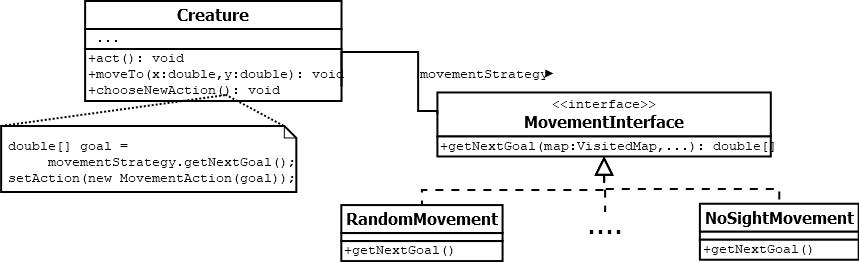
\includegraphics[width=\linewidth]{images/strategy-pattern.png}
	\caption{Strategy Pattern bei der Wegfindung}
\end{figure}

Dass diese Algorithmen zur Laufzeit ersetzt werden können, bietet die Möglichkeit für interessante Kreaturen-Interaktionen und Tower-Arten: Mit dem \class{AmnesiaTower} wurde ein Turm implementiert, der die Creeps durch seine Schüsse verwirrt. Dabei ersetzt er für eine kurze Zeit den eigentlichen Wegfindungsalgorithmus der Kreatur durch \class{RandomMovement}. Genauso könnte man Creeparten implementieren, die anderen beim Kommunizieren bessere Strategien beibringen, also z.B. \class{RandomMovement} der einfachsten Kreaturen durch \class{SightMovement} ersetzen. Ebenfalls angedacht sind Kommandeure, die -- statt selbst durch das Labyrinth zu rennen -- auf Türme klettern und von dort mit Überblick über das gesamte Labyrinth die anderen Creeps durchlotsen können, also die Bewegung durch \class{PerfectMovement} ersetzen. 

Auch Algorithmusimplementierungen, die gar nicht darauf abzielen das Labyrinth zu durchqueren, wären möglich. Beispielsweise könnten intelligentere Kreaturen an geschützten Stellen warten oder priorisiert zu anderen Kreaturen laufen, um diesen Informationen weiterzugeben. Das Projekt bietet hier wie man sieht noch einige Erweiterungen, die bisher noch nicht implementiert werden konnten. Die Grundfunktionalität, um solche Features umzusetzen, sind allerdings mit dem Strategy Pattern gelegt und am Beispiel des Amnesie-Turms auch verwendet.
% subsection strategy_pattern (end)


\subsection{Static Factory Method} % (fold)
\label{sub:static_factory_method}
Gemeint ist hier nicht das Factory Method Pattern, sondern eine statische Methode zur Erzeugung eines Objektes einer Klasse. Im Gegensatz zum Konstruktor hat die Static Factory Method die Möglichkeit auch Objekte von Unterklassen zu erzeugen oder ein bereits erzeugtes Objekt zurückzugeben. In diesem Sinne verwendet z.B. auch das Singleton Pattern eine Static Factory Methode. Dieses Vorgehen wurde sowohl für Türme verwendet, bei denen der Aufruf konkrete Objekte der Unterklassen erzeugt, sowie für die Kreaturen. Bei letzteren ist die Erzeugung etwas umfangreicher und mit verschiedenen Parametern möglich und wurde zur Übersichtlichkeit daher in eine eigene Klasse \class{CreatureFactory} ausgelagert. Diese Factory kann dann z. B. anhand des Types und des Zeitfortschritts die Leben und den Wert der Creeps, sowie deren Bewegungsstrategie bestimmen und entsprechend den Konstruktor der \class{Creature} aufrufen. Dadurch wird die Erzeugung der Figuren besser gekapselt.

% subsection static_factory_method (end)
% section softwaredesign (end)
\newpage
\thispagestyle{empty}
{\Large \textbf{Eidesstattliche Versicherung}}

\textbf{Erklärung zur Hausarbeit gemäß §29 (Abs.6) LPO I}

Hiermit erkläre ich, dass die vorliegende Hausarbeit von mir selbstständig verfasst wurde und dass keine anderen als die angegebenen Hilfsmittel benutzt wurden. Die Stellen der Arbeit, die anderen Werken dem Wortlaut oder Sinn nach entnommen sind, sind in jedem einzelnen Fall unter Angabe der Quelle als Entlehnung kenntlich gemacht. 

Diese Erklärung erstreckt sich auch auf etwa in der Arbeit enthaltene Zeichnungen, Kartenskizzen und bildliche Darstellungen. 

\vspace{2cm}

\begin{tabular}{lcl}
    \hspace{5cm} & \hspace{2cm} & \hspace{7cm} \\
    \dotfill & & \dotfill \\
    Ort, Datum & & Name
\end{tabular}

\end{document}
